\documentclass{article} % For LaTeX2e
\usepackage{nips14submit_e,times}
\usepackage{amsmath}
\usepackage{amsthm}
\usepackage{amssymb}
\usepackage{mathtools}
\usepackage{hyperref}
\usepackage{url}
\usepackage{algorithm}
\usepackage[noend]{algpseudocode}
%\documentstyle[nips14submit_09,times,art10]{article} % For LaTeX 2.09

\usepackage{graphicx}
\usepackage{caption}
\usepackage{subcaption}

\def\eQb#1\eQe{\begin{eqnarray*}#1\end{eqnarray*}}
\def\eQnb#1\eQne{\begin{eqnarray}#1\end{eqnarray}}
\providecommand{\e}[1]{\ensuremath{\times 10^{#1}}}
\providecommand{\pb}[0]{\pagebreak}

\newcommand{\E}{\mathrm{E}}
\newcommand{\Var}{\mathrm{Var}}
\newcommand{\Cov}{\mathrm{Cov}}

\def\Qb#1\Qe{\begin{question}#1\end{question}}
\def\Sb#1\Se{\begin{solution}#1\end{solution}}

\newenvironment{claim}[1]{\par\noindent\underline{Claim:}\space#1}{}
\newtheoremstyle{quest}{\topsep}{\topsep}{}{}{\bfseries}{}{ }{\thmname{#1}\thmnote{ #3}.}
\theoremstyle{quest}
\newtheorem*{definition}{Definition}
\newtheorem*{theorem}{Theorem}
\newtheorem*{lemma}{Lemma}
\newtheorem*{question}{Question}
\newtheorem*{preposition}{Preposition}
\newtheorem*{exercise}{Exercise}
\newtheorem*{challengeproblem}{Challenge Problem}
\newtheorem*{solution}{Solution}
\newtheorem*{remark}{Remark}
\usepackage{verbatimbox}
\usepackage{listings}
\title{Probabilistic Method: \\
Problem Set I}


\author{
Youngduck Choi \\
CIMS \\
New York University\\
\texttt{yc1104@nyu.edu} \\
}


% The \author macro works with any number of authors. There are two commands
% used to separate the names and addresses of multiple authors: \And and \AND.
%
% Using \And between authors leaves it to \LaTeX{} to determine where to break
% the lines. Using \AND forces a linebreak at that point. So, if \LaTeX{}
% puts 3 of 4 authors names on the first line, and the last on the second
% line, try using \AND instead of \And before the third author name.

\newcommand{\fix}{\marginpar{FIX}}
\newcommand{\new}{\marginpar{NEW}}

\nipsfinalcopy % Uncomment for camera-ready version

\begin{document}


\maketitle

\begin{abstract}
This work contains solutions to the problem set I
of Probabilistic Method 2016 at Courant Institute of Mathematical Sciences.
\end{abstract}

\bigskip

\begin{question}[1]
\hfill
\begin{figure}[h!]
  \centering
    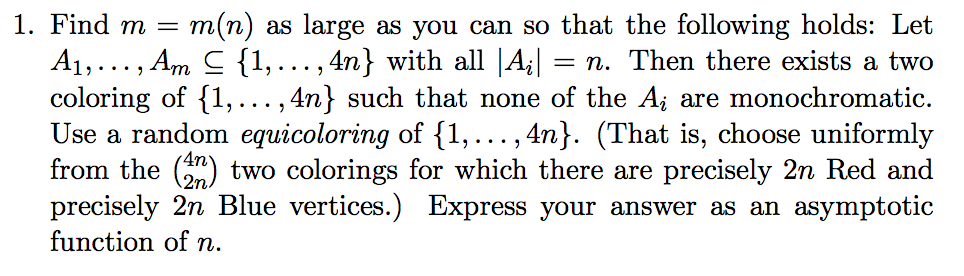
\includegraphics[width=1\textwidth]{pm-1-1.png}
\end{figure}
\end{question}
\begin{solution}
We consider a random equicoloring of $\{1, 2, ..., 4n \}$. Formally, we consider a finite
sample space of all possible equicoloring of $\{1,2,..., 4n\}$, associated with 
a uniform probability, which assigns each outcome in the space with 
$\frac{1}{{4n \choose 2n}}$. First, observe that the probability of the event, where $A_i$ 
is monochromatic is given by
\eQb
P(\{ A_i \text{ is monochromatic} \}) &=& 2\dfrac{{ 3n \choose n}}{{4n \choose 2n}}, 
\eQe
as there are ${3n \choose n}$ cases of coloring the rest of the graph
, when $A_i$ has a fixed monochromatic coloring. 
 By the subadditivity of probability, we have
\eQb
P( \bigcup_{i=1}^{m} \{ A_i \text{ is monochromatic }\} ) 
&\leq& \sum_{i=1}^{m} P(\{A_i \text{ is monochromatic}\}) \\
&=& m \cdot 2\dfrac{{3n \choose n}}{{4n \choose 2n}}.
\eQe
By DeMorgan's laws, we see that
\eQb
(\bigcup_{i=1}^{m} \{ A_i \text{ is monochromatic }\})^c &=& 
\bigcap_{i=1}^{m} \{ A_i \text{ is monochromatic }\}^c \\
&=& \{ \text{No } A_i \text{ is monochromatic} \}. 
\eQe
Since the sum of an event and its complement event is $1$ by one of the axioms of probability,
if we have $m < \dfrac{ {4n \choose 2n } }{2{ 3n \choose n}}$, then 
\eQb
P(\{ \text{No } A_i \text{ is monochromatic} \}) &>& 0. 
\eQe
Now, we express this answer as an asymptotic function of $n$. 
Using Sterling's formula, we have
\eQb
2\dfrac{{3n \choose n}}{{4n \choose 2n}} &=& 2\dfrac{(3n)!(2n)!}{(n!(4n)!} \\
&=& 2\dfrac{(\frac{3n}{e})^{3n}(\frac{2n}{e})^{2n}\sqrt{2\pi(3n)}
\sqrt{2\pi(2n)}}{(\frac{n}{e})^{n}(\frac{4n}{e})^{4n}
\sqrt{2\pi(n)}\sqrt{2\pi(4n)}}(1 + o(1)) \\ 
&=& \sqrt{6}(\dfrac{3}{4})^{3n}(1 + o(1)),
\eQe
as required. It follows that the main asymptotic term on 
the upper bound of $m$ is the $(\dfrac{4}{3})^{3n}$ term, which is 
an exponential function of $n$.  \hfill $\qed$

\end{solution}

\newpage

\begin{question}[2]
\hfill
\begin{figure}[h!]
  \centering
    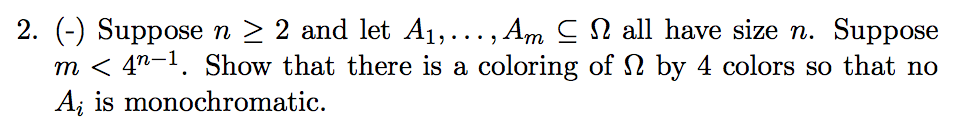
\includegraphics[width=1\textwidth]{pm-1-2.png}
\end{figure}
\end{question}
\begin{solution}
We consider a random vertex 4-coloring of $\Omega$. Formally, we consider a finite
sample space of all possible vertex 4-coloring of $\Omega$, associated with a uniform
probability, which assigns each outcome in the space with $\frac{1}{|\Omega |}$ probability.
By the subadditivity of probability, we have
\eQb
P( \bigcup_{i=1}^{m} \{ A_i \text{ is monochromatic }\} ) 
&\leq& \sum_{i=1}^{m} P(\{A_i \text{ is monochromatic}\}) \\
&=& m \cdot 4^{1 - n}.
\eQe
As $m < 4^{n-1}$, it follows that
\eQb
m \cdot 4^{1 - n} &<& 4^{n-1} \cdot 4^{1-n} = 1,
\eQe
which primarily grants us
\eQb
P( \bigcup_{i=1}^{m} \{ A_i \text{ is monochromatic }\} ) < 1. 
\eQe
By DeMorgan's laws, we see that
\eQb
(\bigcup_{i=1}^{m} \{ A_i \text{ is monochromatic }\})^c &=& 
\bigcap_{i=1}^{m} \{ A_i \text{ is monochromatic }\}^c \\
&=& \{ \text{No } A_i \text{ is monochromatic} \}. 
\eQe
Since the sum of an event and its complement event is $1$ by one of the axioms of probability,
we have shown that
\eQb
P(\{ \text{No } A_i \text{ is monochromatic} \}) &>& 0. 
\eQe
Hence, we have
shown that there is a coloring of $\Omega$ by 4 colors such that no $A_i$ is monochromatic. 
\hfill $\qed$ 

\end{solution}

\newpage

\begin{question}[3]
\hfill
\begin{figure}[h!]
  \centering
    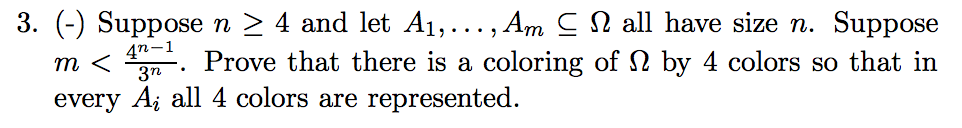
\includegraphics[width=1\textwidth]{pm-1-3.png}
\end{figure}
\end{question}
\begin{solution}
We consider a random vertex 4-coloring of $\Omega$. Formally, we consider a finite
sample space of all possible vertex 4-coloring of $\Omega$, associated with a uniform
probability, which assigns each outcome in the space with $\frac{1}{|\Omega |}$ probability.
By the subadditivity of probability, we have
\eQb
P( \bigcup_{i=1}^{m} \{ A_i \text{ has at most 3 colors }\} ) 
&\leq& \sum_{i=1}^{m} P(\{ A_i \text{ has at most 3 colors } \}) \\
&\leq& m \cdot 3^n 4^{-n+1},
\eQe
as there are ${ 4 \choose 1 } 3^n$ is an upper bound to 
ways to have coloring of at most 3 colors for $n$ vertices.  
Since $m < 3^{-n}4^{n-1}$, it follows that
\eQb
m \cdot 3^{n}4^{-n+1}  &<& 3^{-n} 4^{n-1} 3^n 4^{-n+1} = 1,
\eQe
which primarily grants us
\eQb
P( \bigcup_{i=1}^{m} \{ A_i \text{ has at most 3 colors }\} ) < 1. 
\eQe
By DeMorgan's laws, we see that
\eQb
(\bigcup_{i=1}^{m} \{ A_i \text{ has at most 3 colors }\})^c &=& 
\bigcap_{i=1}^{m} \{ A_i \text{ has at most 3 colors }\}^c \\
&=& \{ \text{Every } A_i \text{ has 4 colors} \}. 
\eQe
Since the sum of an event and its complement event is $1$ by one of the axioms of probability,
we have shown that
\eQb
P(\{ \text{Every } A_i \text{ has 4 colors } \}) &>& 0. 
\eQe
Hence, we have
shown that there is a coloring of $\Omega$ by 4 colors such that every $A_i$ has 4 colors. 
\hfill $\qed$ 
\end{solution}

\newpage

\begin{question}[4]
\hfill
\begin{figure}[h!]
  \centering
    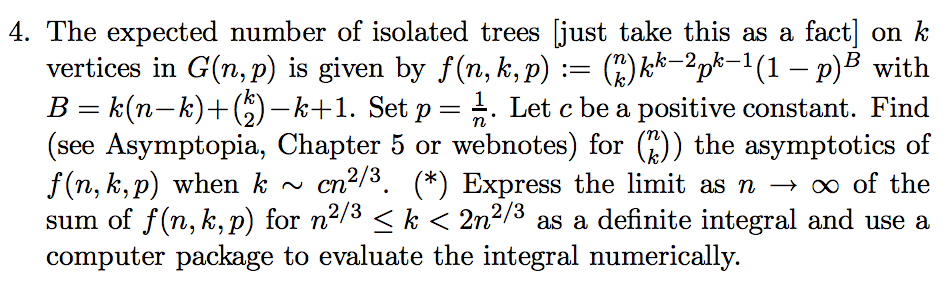
\includegraphics[width=1\textwidth]{pm-1-4.png}
\end{figure}
\end{question}
\begin{solution}
First of all the problem can be found in the book, Asymptopia.
We note that $k \sim c n^{\frac{2}{3}}$, thus $k = o(n^{\frac{3}{4}})$.
Then, by the case 4 of the result in $5.1$ Asymtopia, with Stirling's formula, we have
\eQb
{n \choose k} &\sim& 
e^{-\frac{k^2}{2n}} e^{-\frac{k^3}{6n^2}}\dfrac{n^k}{k!} \\
&\sim& 
e^{-\frac{k^2}{2n}} e^{-\frac{k^3}{6n^2}}n^k \dfrac{e^k}{n^k \sqrt{2\pi k}} \\
\eQe
Now, by direct computation, it follows that
\eQb
B &=& k(n-k) + {k \choose 2} - k + 1 \\
&=& kn - \dfrac{1}{2}k^2 - \dfrac{3}{2} + 1 \\
&=& kn - \dfrac{1}{2}k^2 + O(k),
\eQe
which then yields
\eQb
ln[(1-p)^{k(n-k) + {k \choose 2} - (k-1)}] &=& -k + \dfrac{k^2}{2n} + o(1).
\eQe
Now, substituting the above into the first asyptomtic equivalence we have established, we have
\eQb
f(n,k,p) &\sim& e^{-\frac{c^3}{6}}n^{-\frac{2}{3}}c^{-\frac{5}{2}}(2\pi)^{-\frac{1}{2}}, 
\eQe
as required. \hfill $\qed$
\end{solution}

\newpage

\begin{question}[5]
\hfill
\begin{figure}[h!]
  \centering
    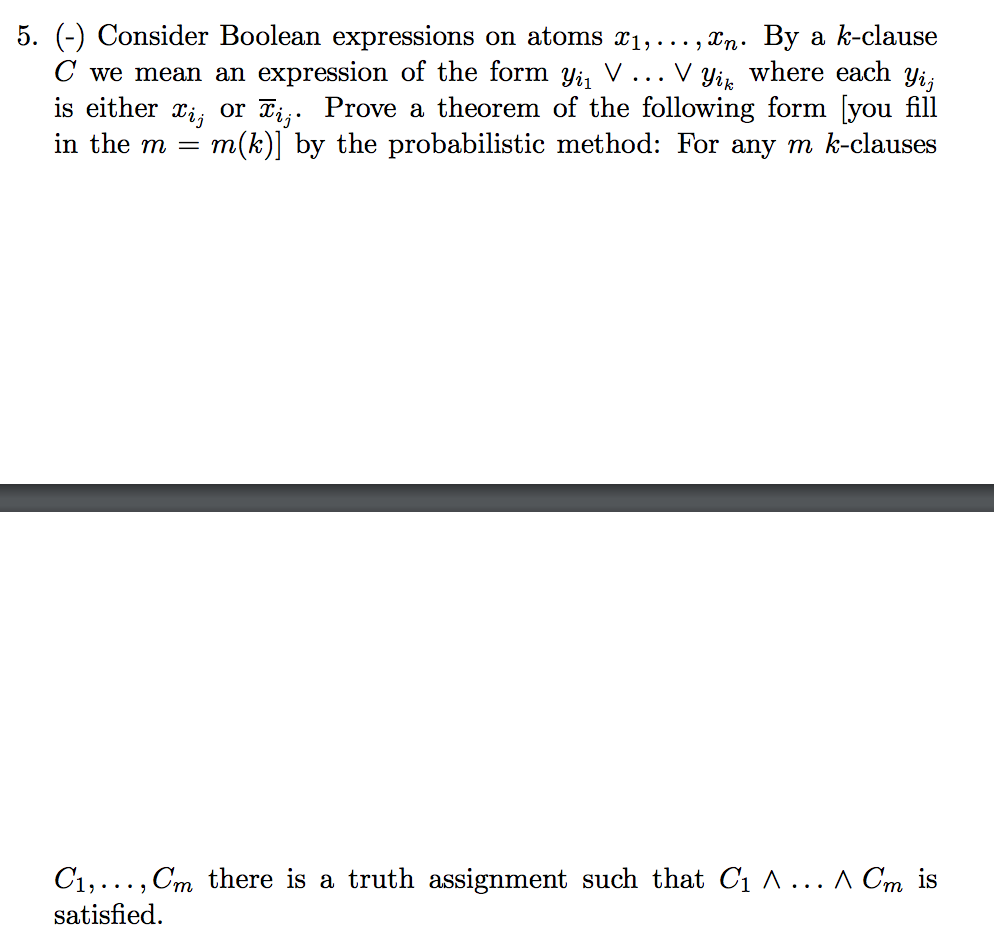
\includegraphics[width=1\textwidth]{pm-1-5.png}
\end{figure}
\end{question}
\begin{solution}
We claim the following: Suppose $m < 2^{k}$. Then, there exists a truth assignment
such that $\bigvee_{i=1}^{m} C_i$ is satisfied.

\bigskip

We consider a random truth assignment of atoms, $\{ x_1, ... x_n\}$. Formally,
we consider a finite sample space of all possible truth assignment of atoms,
associated with a uniform probability, which assigns each outcome in the space
with $\frac{1}{2^n}$ probability.  
By the subadditivity of probability, we have
\eQb
P( \bigcup_{i=1}^{m} \{ C_i \text{ is not satisfied }\} ) 
&\leq& \sum_{i=1}^{m} P(\{ C_i \text{ is not satisfied } \}) \\
&\leq& m \cdot 2^{-k},
\eQe
as there is only one assignment, which assigns all false values to $k$ variables, 
that makes $C_i$ clause not satisfied. 
Since $m < 2^{k}$, it follows that
\eQb
m \cdot 2^{-k} < 2^{k} 2^{-k} = 1,
\eQe
which primarily grants us
\eQb
P( \bigcup_{i=1}^{m} \{ C_i \text{ is not satisfied }\} ) < 1. 
\eQe
By DeMorgan's laws, we see that
\eQb
(\bigcup_{i=1}^{m} \{ C_i \text{ is not satisfied }\})^c &=& 
\bigcap_{i=1}^{m} \{ C_i \text{ is not satisfied }\}^c \\
&=& 
\bigcap_{i=1}^{m} \{ C_i \text{ is satisfied } \} 
= \{ \bigvee C_i \text{ is satisfied } \}. 
\eQe
Since the sum of an event and its complement event is $1$ by one of the axioms of probability,
we have shown that
\eQb
P(\{ \bigvee_{i=1}^{m}  C_i \text{ is satisfied } \}) &>& 0. 
\eQe
Hence, we have
shown that there is a truth assignment such that  
$\bigvee_{i=1}^{m} C_i$ is satisfied, when $m < 2^k$. 

\hfill $\qed$ 
 
\end{solution}

\newpage

\end{document}
